%
% File naacl2019.tex
%
%% Based on the style files for ACL 2018 and NAACL 2018, which were
%% Based on the style files for ACL-2015, with some improvements
%%  taken from the NAACL-2016 style
%% Based on the style files for ACL-2014, which were, in turn,
%% based on ACL-2013, ACL-2012, ACL-2011, ACL-2010, ACL-IJCNLP-2009,
%% EACL-2009, IJCNLP-2008...
%% Based on the style files for EACL 2006 by
%%e.agirre@ehu.es or Sergi.Balari@uab.es
%% and that of ACL 08 by Joakim Nivre and Noah Smith

\documentclass[11pt,a4paper]{article}
\usepackage{authblk}
\usepackage[hyperref]{naaclhlt2019}
\usepackage{times}
\usepackage{latexsym}
\usepackage{todonotes}
\usepackage{url}
\usepackage{color}
\usepackage[utf8]{inputenc}
\usepackage{flushend}
\usepackage{booktabs}
\usepackage{hyperref}

\aclfinalcopy % Uncomment this line for the final submission
\def\aclpaperid{*} %  Enter the acl Paper ID here

%\setlength\titlebox{5cm}
% You can expand the titlebox if you need extra space
% to show all the authors. Please do not make the titlebox
% smaller than 5cm (the original size); we will check this
% in the camera-ready version and ask you to change it back.

\newcommand\BibTeX{B{\sc ib}\TeX}

\title{Overview of the eHealth Knowledge Discovery Challenge at IberLEF 2019}

\author[1]{\textbf{A. Piad-Morffis}}
\author[2]{\textbf{Y. Gutiérrez}}
\author[1]{\textbf{J. P. Consuegra-Ayala}}
\author[1]{\textbf{S. Estevez-Velarde}}
\author[3]{\\\textbf{R. Muñoz}}
\author[3]{\textbf{A. Montoyo}}
\author[1]{\textbf{Y. Almeida}}
\affil[1]{School of Math and Computer Science, University of Havana}
\affil[ ]{ \texttt{\{apiad,sestevez,jpconsuegra,yudy\}@matcom.uh.cu} }
%  }
\affil[2]{University Institute for Computing Research (IUII), University of Alicante}
\affil[3]{Deparment of Software and Computing Systems, University of Alicante}
\affil[ ]{ \texttt{\{ygutierrez,rafael,montoyo\}@dlsi.ua.es} }

% \author{Alejandro Piad-Morffis \\
%   University of Havana \\
%   {\tt apiad@matcom.uh.cu} \\\And
%   Yoan Gutiérrez \\
%   University of Alicante \\
%   {\tt ygutierrez@dlsi.ua.es} \\
%   \And
%   Suilan Estevez-Velarde \\
%   University of Havana \\
%   {\tt sestevez@matcom.uh.cu} \\
%   \And
%   Rafael Muñoz \\
%   University of Alicante \\
%   {\tt rafael@dlsi.ua.es} \\}


\date{}

\renewcommand\Authands{, }

\begin{document}
\maketitle

\newcommand\github{https://github.com/knowledge-learning/satr-ann}

\newcommand{\td}[1]{\todo[inline, color=green]{\texttt{-} #1}}
\newcommand{\qs}[1]{\todo[inline, color=yellow]{\texttt{?} #1}}
\newcommand{\er}[1]{\todo[inline, color=red]{\texttt{!} #1}}
\newcommand{\nt}[1]{{\color{orange}\texttt{*} #1}}

\begin{abstract}
\end{abstract}

\section{Introduction}

\todo[inline, color=green]{$<$REWRITE$>$: Taken from NAACL paper}
Knowledge discovery is a field of computer science that shows an accelerated growth in the past three decades.
Advances in this area have been applied in many domains, from databases~\cite{fayyad1996data, knowledgeDatabase} to
images~\cite{lu2016visual} and natural language text~\cite{carlson2010toward}.
Specifically in natural language text, this field is highly relevant in the biomedical and health domains,
where it is used for performing tasks such as
Named Entity Recognition~(NER), Relationship Extraction and Hypothesis Generation, among others~\cite{simpson2012biomedical}.
These tasks generally use annotated corpora for learning the characteristics that appear in the text and mapping them to knowledge structures.
For each task, specific annotation models have been designed that focus on specific elements of the text.
For example, in NER tasks is more important to focus on nominal phrases than other grammatical constructions.

Despite that these domain-specific tasks are different, most of them share common characteristics. For example, most tasks deal with the detection of relevant entities and their relations. Hence, promoting general-purpose annotation models would allow the design of reusable and cross-domain knowledge discovery techniques.
In this line, several domain-independent semantic representations have been developed~(e.g., AMR~\cite{amr}, PropBank~\cite{propbank}, FrameNet~\cite{framenet}).
However, these representations rely heavily on fine-grained lexicons that define specific semantic roles for each word meaning. Therefore, developing knowledge discovery systems with this level of detail supposes great challenges. Using more coarse-grained semantic representation, even with the loss of some representational capacity, would simplify the creation of automatic techniques based on machine learning.
This representation could also be used as the first stage in a pipeline for a domain-specific task, thus reusing resources and techniques in domains with few available resources.
\todo[inline, color=green]{$<$/REWRITE$>$}

\todo[inline, color=blue]{MOTIVATION. Develop a general-purpose annotation model, corpora and related algorithms for KD in eHealth.}

The field of eHealth is a research area with a important number of publication.
For this reason is interests for textual analysis, in particular for knowledge
discovery. In eHealth text appear concept that represent important concepts such as
enfermedades, tratamientos, etc.
But in many case the problem of recognize this concept is specif and depend of the domain.
The objective of this challenge is propose a general task for knowledge discovery in eHealth domain. Where....

\todo[inline, color=blue]{RELATED WORKS. Other KD extraction tasks. Previous eHealth-KD challenge.}

This proposal is inspired in a theoretical combination between teleologies and the extraction action proposed in ICAI congress....
The antecedent of this proposal is a challenge of TASS in 2018 where.... is proposed...
The mayor difference are....

\section{Challenge description}\label{sec:sota}

\todo[inline, color=blue]{Why divide in two tasks.}

\subsection{Subtask A: Key phrase Extraction and Classification}\label{sec:taskA}

\todo[inline]{REWRITE: Taken from website}

Given a list of eHealth documents written in Spanish, the goal of this subtask is to identify all the key phrases per document and their classes. These key phrases are all the relevant terms (single word or multiple words) that represent semantically important elements in a sentence. Figure~\ref{fig:subtaskA} shows the relevant key phrases that appear in an example set of sentences.

\begin{figure}[htbp]
    \centering
    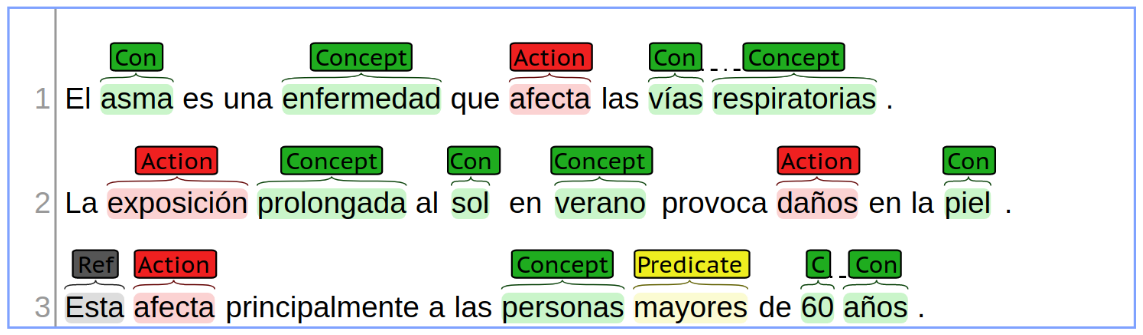
\includegraphics[width=\columnwidth]{task_a.png}
    \caption{Annotation of the relevant key phrases and associated classes in a set of example sentences.}
    \label{fig:subtaskA}
\end{figure}

Note that some key phrases (``\textit{vías respiratorias}'' and ``\textit{60 años}'') span more than one word. Key phrases always consist of one or more complete words (i.e., not a prefix or a suffix of a word), and will never include any surrounding punctuation symbols.
There are four categories or classes for key phrases:

\begin{description}
    \item[Concept:] a general category that indicates the key phrase is a relevant term, concept, idea, in the knowledge domain of the sentence.

    \item[Action:] a concept that indicates a process or modification of other concepts. It can be indicated by a verb or verbal construction, such as ``\textit{afecta}''~(affects), but also by nouns, such as ``\textit{exposición}''~(exposition), where it denotes the act of being exposed to the Sun, and ``\textit{daños}''~(damages), where it denotes the act of damaging the skin. It can also be used to indicate non-verbal functional relations, such as ``\textit{padre}''~(parent).

    \item[Predicate:] used to represent a function or filter of another set of elements, which has a semantic label in the text, such as ``\textit{mayores}''~(older), and is applied to a concept, such as ``\textit{personas}''~(people) with some additional arguments such as ``\textit{60 años}''~(60 years).

    \item[Reference:] A textual element that refers to a concept --of the same sentence or of different one--, which can be indicated by textual clues such as ``\textit{esta}'', ``\textit{aquel}'', and similar.
\end{description}

The input for Subtask A is a text document with a sentence per line. All sentences have been tokenized at the word level (i.e., punctuation signs, parenthesis, etc, are separated from the surrounding text).

\todo[inline, color=blue]{Brief explanation of the entity types. Cite NAACL paper.}

\subsection{Subtask B: Relation Extraction}\label{sec:taskB}

Subtask B continues from the output of Subtask A, by linking the key phrases detected and labeled in each document. The purpose of this subtask is to recognize all relevant semantic relationships between the entities recognized. Eight of the thirteen semantic relations defined for this challenge can be identified in figure~\ref{fig:subtaskB}

\begin{figure}[htbp]
    \centering
    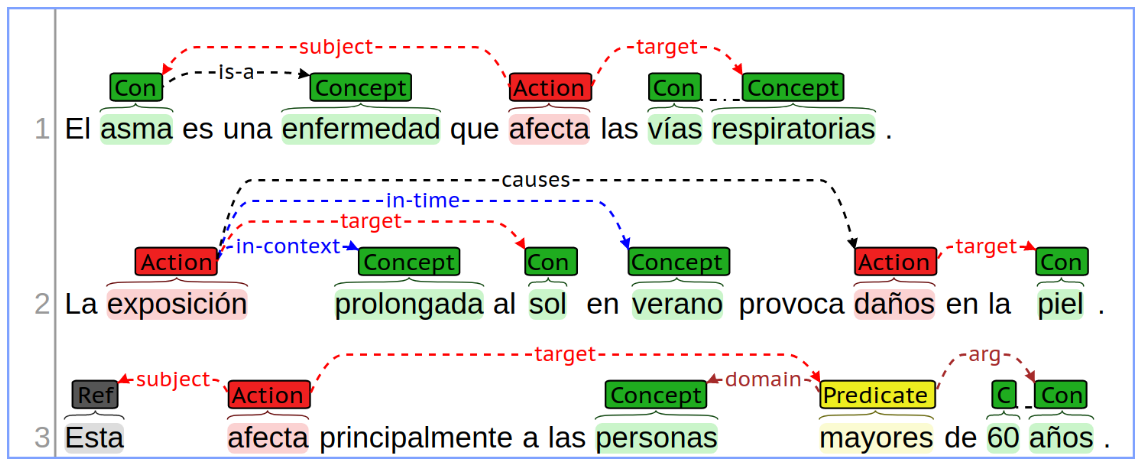
\includegraphics[width=\columnwidth]{task_b.png}
    \caption{Annotation of the relevant semantic relations in an set of example sentences.}
    \label{fig:subtaskB}
\end{figure}

The semantic relations are divided in different categories:

\begin{description}
    \item[General relations (6):] general-purpose relations between two concepts that have a specific semantic:

    \begin{description}
        \item[is-a:] indicates that one concept is a sub-type, instance, or member of the class identified by the other.
        \item[same-as:] indicates that two concepts are semantically the same.
        \item[has-property:] indicates that one concept has a given property or characteristic.
        \item[part-of:] indicates that a concept is a constituent part of another.
        \item[causes:] indicates that one concept provokes the existence or occurrence of another.
        \item[entails:] indicates that the existence of one concept implies the existence or occurrence of another.

    \end{description}

    \item[Contextual relations (3):] allow to refine a concept by attaching the following modifiers:

    \begin{description}
        \item[in-time:] to indicate that something exists, occurs or is confined to a time-frame, such as in ``\textit{exposición}'' in-time ``\textit{verano}''.
        \item[in-place:] to indicate that something exists, occurs or is confined to a place or location.
        \item[in-context:] to indicate a general context in which something happens, like a mode, manner, or state, such as ``\textit{exposición}'' in-context ``\textit{prolongada}''.
    \end{description}

    \item[Action roles (2):] indicate which role plays the concepts related to an Action:

    \begin{description}
        \item[subject:] indicates who performs the action, such as in ``\textit{[el] asma afecta [...]}''.
        \item[target:] indicates who receives the effect of the action, such as in ``\textit{[...] afecta [las] vías respiratorias}''.
    \end{description}

    \item[Predicate roles (2):] indicate which role plays the concepts related to a Predicate:

    \begin{description}
        \item[domain:] indicates the main concept on which the predicate applies.
        \item[arg:] indicates additional arguments that further specify the predicate.
    \end{description}
\end{description}

\todo[inline, color=blue]{Brief explanation of the relation types. Cite NAACL paper.}

The input for Subtask B consists of plain text and the output for Subtask A, i.e., the span limits for each key phrase and the corresponding class.

\subsection{Evaluation Metrics}

The challenge proposed a main evaluation scenario (Scenario 1) where both subtasks previously described are performed in sequence. The submission that obtained the highest F1 score for the Scenario 1 was considered the best overall performing system of the challenge. Additionally, participants had have the opportunity to address specific subtasks by submitting to two optional scenarios, once for each subtask. These two additional scenarios measure the performance in individual subtasks independently of each other.

The Scenario 1 is more complex than solving each optional scenario separately, since errors in subtask A will necessary translate to errors in subtask B. For this reason it is considered the main evaluation metric. Additionally, this scenario also provides the possibility for integrated end-to-end solutions that solve both subtask simultaneously.

\subsubsection{Main Evaluation (Scenario 1)}

This scenario evaluates all of the subtasks together as a pipeline. The input consists only of a plain text, and the expected output will be the two output files for Subtask A and B, as described before. The measures will be precision, recall and F1 as follows:

$$Rec_{AB} = \frac{C_A + C_B + \frac{1}{2} P_A}{C_A + I_A + C_B + P_A + M_A + M_B} $$

$$Prec_{AB} = \frac{C_A + C_B + \frac{1}{2} P_A}{C_A + I_A + C_B + P_A + S_A + S_B} $$

$$F_{1AB} = 2 \cdot \frac{Prec_{AB} \cdot Rec_{AB}}{Prec_{AB} + Rec_{AB}} $$

The exact definition of Correct, Missing, Spurious, Partial and Incorrect is presented in the following sections for each subtask.

\subsubsection{Optional Subtask A (Scenario 2)}

This scenario only evaluates Subtask A. To compute the scores we define correct, partial, missing, incorrect and spurious matches. A brief description about the metrics follows:

\begin{description}
    \item[Correct:] are reported when a text span in a submission matches exactly with a corresponding text span in the gold file. Only one correct match per entry in the gold file can be matched. Hence, duplicated entries will count as Spurious.
    \item[Incorrect:] are reported when text span values match, but not the associated class.
    \item[Partial:] are reported when two text span intervals have a non-empty intersection, such as the case of ``vías respiratorias'' and ``respiratorias'' in the previous example (and matching class). Notice that a partial phrase will only be matched against a single correct phrase, to discourage a few large text spans that cover most of the document from getting a very high score.
    \item[Missing:] are those that appear in the gold file but not in the submission.
    \item[Spurious:] are those that appear in the submission but not in the gold file.
\end{description}

From these definitions, we compute precision, recall, and a standard F1 measure as follows:

$$Rec_{A} = \frac{C_A + \frac{1}{2} P_A}{C_A + I_A + P_A + M_A} $$

$$Prec_{A} = \frac{C_A + \frac{1}{2} P_A}{C_A + I_A + P_A + S_A} $$

$$F_{1A} = 2 \cdot \frac{Prec_{A} \cdot Rec_{A}}{Prec_{A} + Rec_{A}} $$

A higher precision means that the number of spurious identifications is smaller compared to the number of missing identifications, and a higher recall means the opposite. Partial matches are given half the score of correct matches, while missing and spurious identifications are given no score.

\subsubsection{Optional Subtask B (Scenario 3)}

This scenario only evaluates Subtask B. The input is plain text and the correct outputs from Subtask A. Similarly to previous scenarios, we define the correct, missing and spurious items, defined as follows:

\begin{description}
    \item[Correct:] relationships that matched exactly to the gold file, including the class and the corresponding key phrases.
    \item[Missing:] relationships that are in the gold file but not reported in the submission, either because the relation type is wrong, or because one of the arguments didn’t match.
    \item[Spurious:] relationships that are in the submission file but not in the gold file, either because the relation type is wrong, or because one of the arguments didn’t match.
\end{description}

We define standard precision, recall and F1 metrics as follows:

$$Rec_{B} = \frac{C_B}{C_B + M_B} $$

$$Prec_{B} = \frac{C_B}{C_B + S_B} $$

$$F_{1B} = 2 \cdot \frac{Prec_{B} \cdot Rec_{B}}{Prec_{B} + Rec_{B}} $$

\todo[inline, color=blue]{Overall metrics and subtask metrics.}

\subsection{Corpus Description}

\todo[inline, color=blue]{Basic statistics of the corpus}

\section{Systems Description}\label{sec:desc}

\todo[inline, color=blue]{General description of the systems and challenges.}

In the challenge are presented 10 different team with dissimilar proposals of algorithms. The approach used in this system are: knowledge based, machine learning and deep learning.
This section briefly describes each participant system.

To simplify the comparison an better understand the characteristics of each system, we define the following tags to describe the kind of techniques used by each participant:

\begin{description}
    \item[K:] Knowledge Bases;
    \item[S:] Shallow supervised methods (e.g., logistic regression, SVM, Markov models, CRF, \ldots);
    \item[D:] Deep supervised methods (e.g, CNNs, LSTMs, \ldots);
    \item[U:] Unsupervised methods (e.g. clustering or dimensionality reduction techniques, \ldots);
    \item[E:] Embeddings (e.g., Word2Vec, FastText, BERT, ELMo, \ldots);
    \item[N:] Standard NLP techniques (Pos-tagging, AMR parsing, dependency parsing, NER, \ldots); and
    \item[R:] Hand-crafted rules.
\end{description}

\todo[inline, color=blue]{Description of each system.}

\section{Results}

\begin{table}[tb]\centering
    \begin{tabular}{llccc}
        \toprule
        Team         & Tags  & Scn 1     & Scn 2     & Scn 3     \\
        \midrule
        Talp         &       & \bf 0.639 & \bf 0.820 & \bf 0.626 \\
        Ncatala      &       & \bf 0.621 &     0.787 & \bf 0.493 \\
        Abravo       &       & \bf 0.581 & \bf 0.816 &     0.229 \\
        Lsi\_uned    &       &     0.547 &     0.754 & \bf 0.533 \\
        Hulat-TaskAB &       &     0.541 &     0.775 &     0.123 \\
        Uhmajakd     &       &     0.518 & \bf 0.815 &     0.433 \\
        Lsi2\_uned   &       &     0.493 &     0.731 &     0.123 \\
        Iakesg       &       &     0.486 &     0.682 &     0.435 \\
        Baseline     &       &     0.430 &     0.546 &     0.123 \\
        Jlcuad       &       &     0.430 &     0.790 &     0.123 \\
        Vsp          &       &     0.428 &     0.546 & \bf 0.493 \\
        \bottomrule
    \end{tabular}
    \caption{Results (F1 metric) in each scenario, sorted by Scenario 1. The top three (four) results per scenario are highlighted in \textbf{bold}.}
\end{table}

\todo[inline, color=blue]{Qualitative comments on the best results per scenario.}

\subsection{Analysis of Systems Performance}

In this section we present an analysis of the performance of participant systems with respect to three qualitative criteria. First, we analyze the characteristics (as defined by the tags in Section~\ref{sec:desc}) that are correlated with a higher performance in each scenario. Next, we analyze the most common errors in each subtask. Finally, we build an ensemble with the best performing systems and deploy it in the main scenario to compare its performance with the rest of the systems.

\todo[inline, color=blue]{Correlation of tags per subtask.}
\todo[inline, color=blue]{Errors for each entity class and relation.}
\todo[inline, color=blue]{Ensemble description and results.}

\section{Discussion}

\section{Conclusions and Future Work}

\section*{Acknowledgments}

\todo[inline, color=red]{REVIEW}

\textbf{Funding}: This research has been supported by a Carolina Foundation grant in agreement with University of Alicante and University of Havana. Moreover, it has also been partially funded by both aforementioned universities and the Generalitat Valenciana (Conselleria d’Educació, Investigació, Cultura i Esport) through the projects PROMETEO/2018/089, PROMETEU/2018/089;  Social-Univ 2.0 (ENCARGO-INTERNOOMNI-1); and PINGVALUE3-18Y.

The authors would like to thank the team of annotators from the School of Math and Computer Science, at the University of Havana.

% This version of the paper takes into account helpful comments provided by the anonymous reviewers.

\bibliography{naaclhlt2019}
\bibliographystyle{plain}

\appendix

\end{document}
